\newpage

\section{Available Expressions Analysis}

\subsection{Motivation}

Programs may contain code whose result is needed, but in which some computation is simply a redundant
repetition of earlier computation within the same program. The concept of expression availability is useful in dealing with this situation.


\subsection{Backgroud Knowledge}

Any given program contains a finite number of expressions (i.e. computations which potentially
produce values),so we may talk about the set of all expressions of a program. Consider the program in
\ref{lst:expression1}




\begin{lstlisting}[language=C,frame=single, caption=An simple example containing some expressions ,label = lst:expression1]
    int z = x * y; 
    print s + t; 
    int w = u / v;
\end{lstlisting}


This program contian expression \texttt{x*y,s+t,u/v}.



\subsection{Problem Formulation}


Availability is a data-flow property of expressions: “Has the value of this expression already been computed?”
At each instruction, each expression in the programis either available or unavailable. So each instruction(or node of the flowgraph) has
an associated set of available expression.



\subsection{Semantic vs. Syntactic}

An expression is \textit{semantically} available at a node n if its value gets computed
(and not subsequently invalidated) along every execution sequence ending at n.

\begin{figure}[!htb]
	\minipage{0.5\textwidth}
	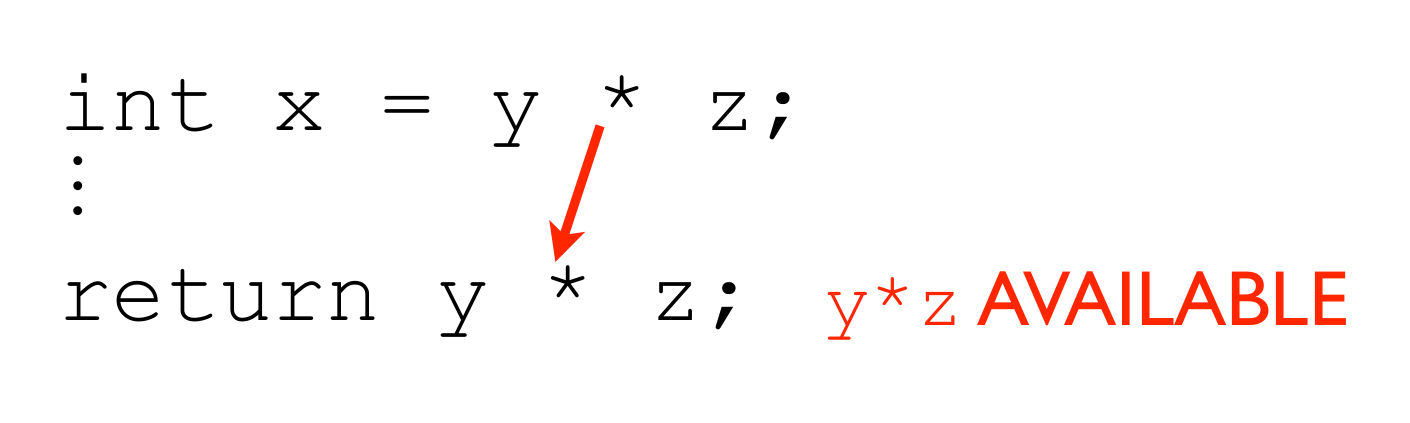
\includegraphics[width=\linewidth]{p1.png}
	\caption{Available expression example}\label{fig:p1}
	\endminipage\hfill
	\minipage{0.5\textwidth}
	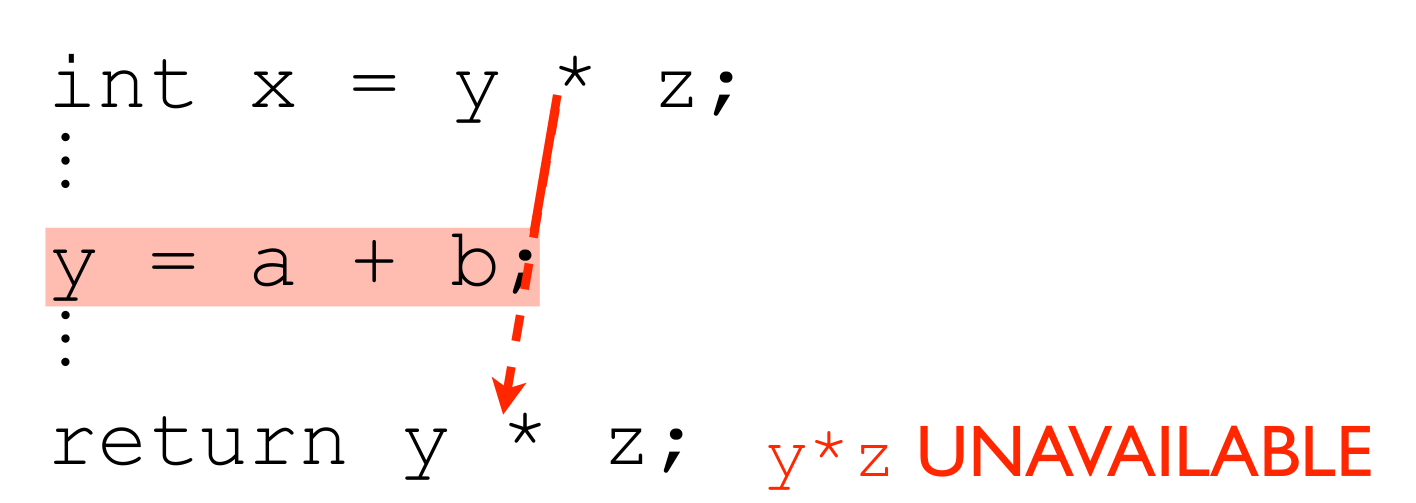
\includegraphics[width=\linewidth]{p2.png}
	\caption{unavailable expression example}\label{fig:p2}
	\endminipage
\end{figure}


An expression is \textit{syntactically} available at a node n if its value gets computed
(and not subsequently invalidated) along every path from the entry of the flowgraph to n.


\begin{figure}[!htb]
	\minipage{0.5\textwidth}
	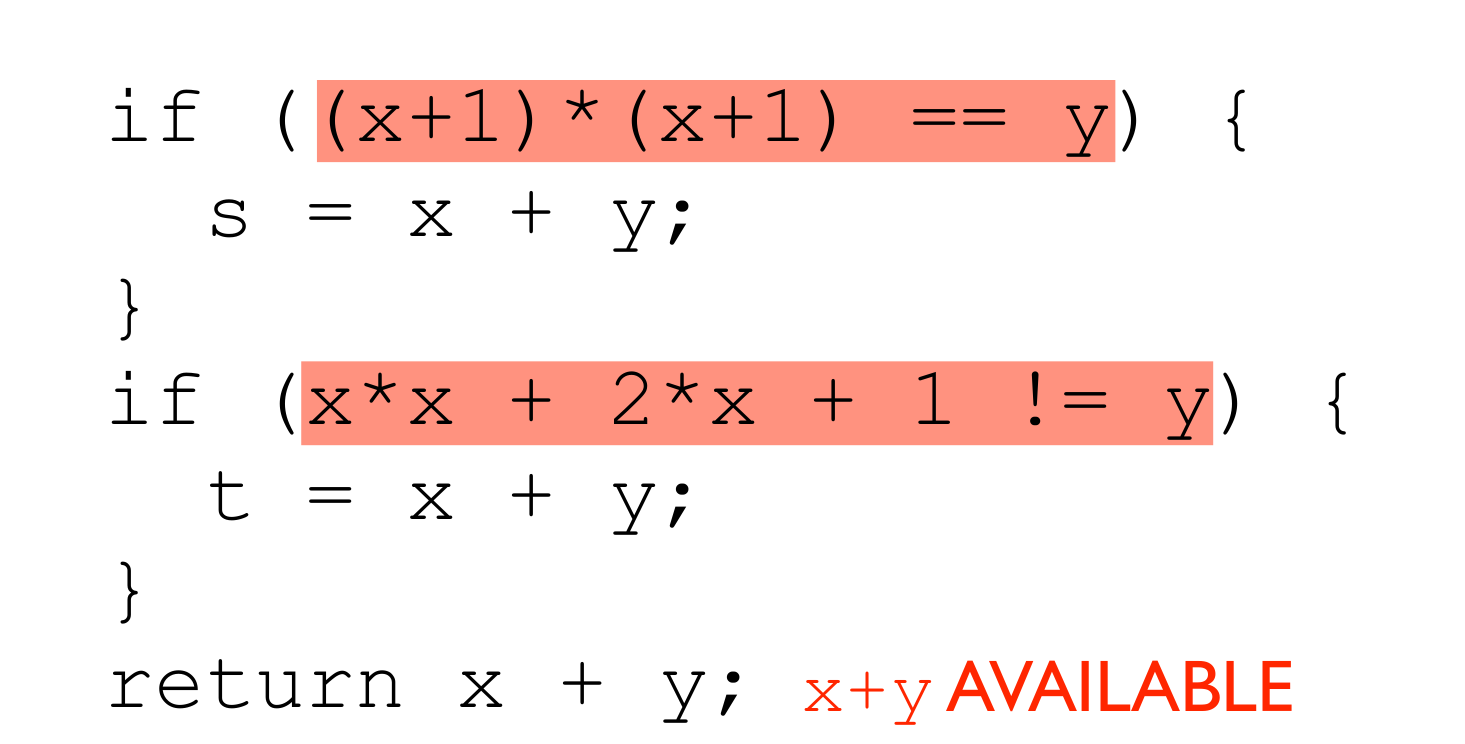
\includegraphics[width=\linewidth]{p4.png}
	\caption{x+y is semantically available}\label{fig:p4}
	\endminipage\hfill
	\minipage{0.4\textwidth}
	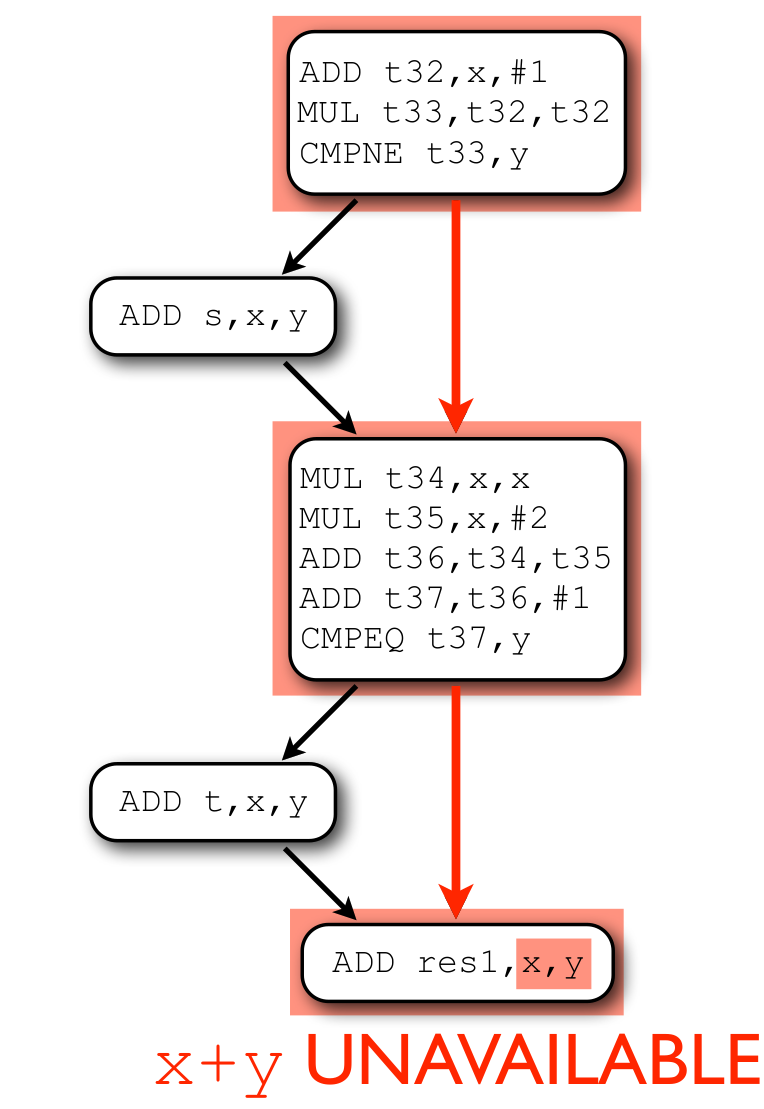
\includegraphics[width=\linewidth]{p3.png}
	\caption{x+y is syntactically unavailable}\label{fig:p3}
	\endminipage
\end{figure}


On the path in red from Figure \ref{fig:p3} through the flowgraph, \(x+y\) is only
computed once, so \(x+y\) is syntactically unavailable at the last instruction.


Whereas with live variable analysis we found safety in assuming that
more variables were live, here we find safety in assuming that fewer
expressions are available. Because if an expression is deemed to be available, we
may do something dangerous (e.g. remove an instruction which recomputes its value).
So sometimes safe means more, but sometimes means less.

\begin{figure}[H]
	\minipage{0.5\textwidth}
	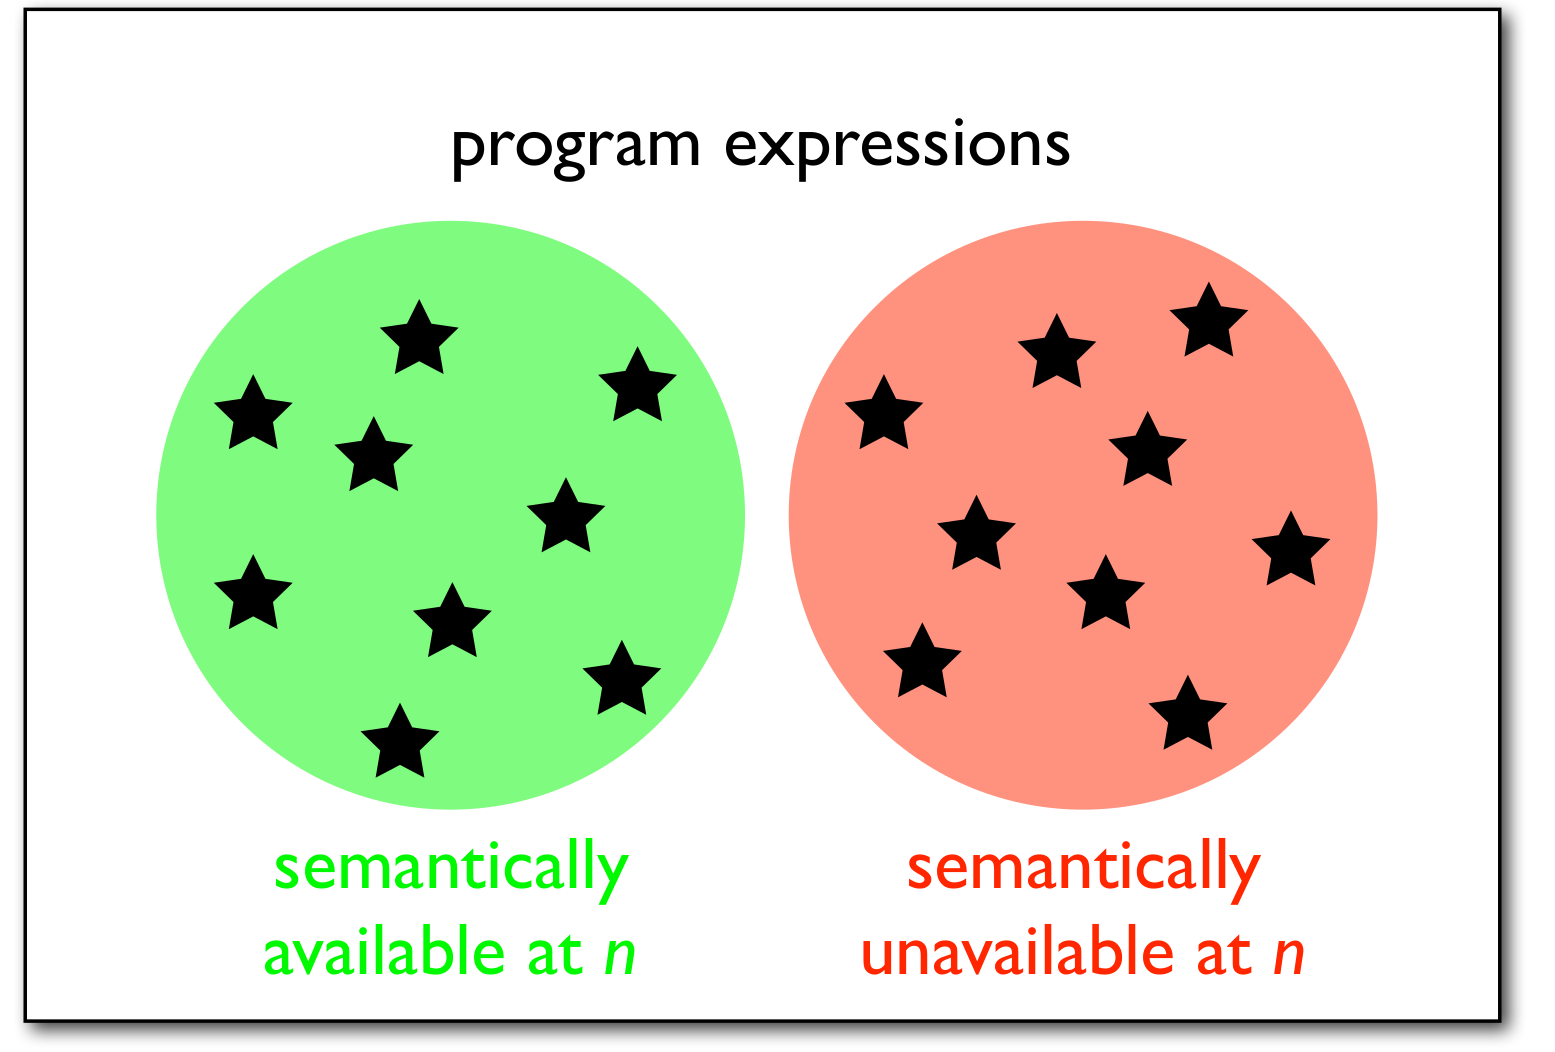
\includegraphics[width=\linewidth]{p5.png}
	\caption{Semantic vs. syntactic}\label{fig:p5}
	\endminipage\hfill
	\minipage{0.5\textwidth}
	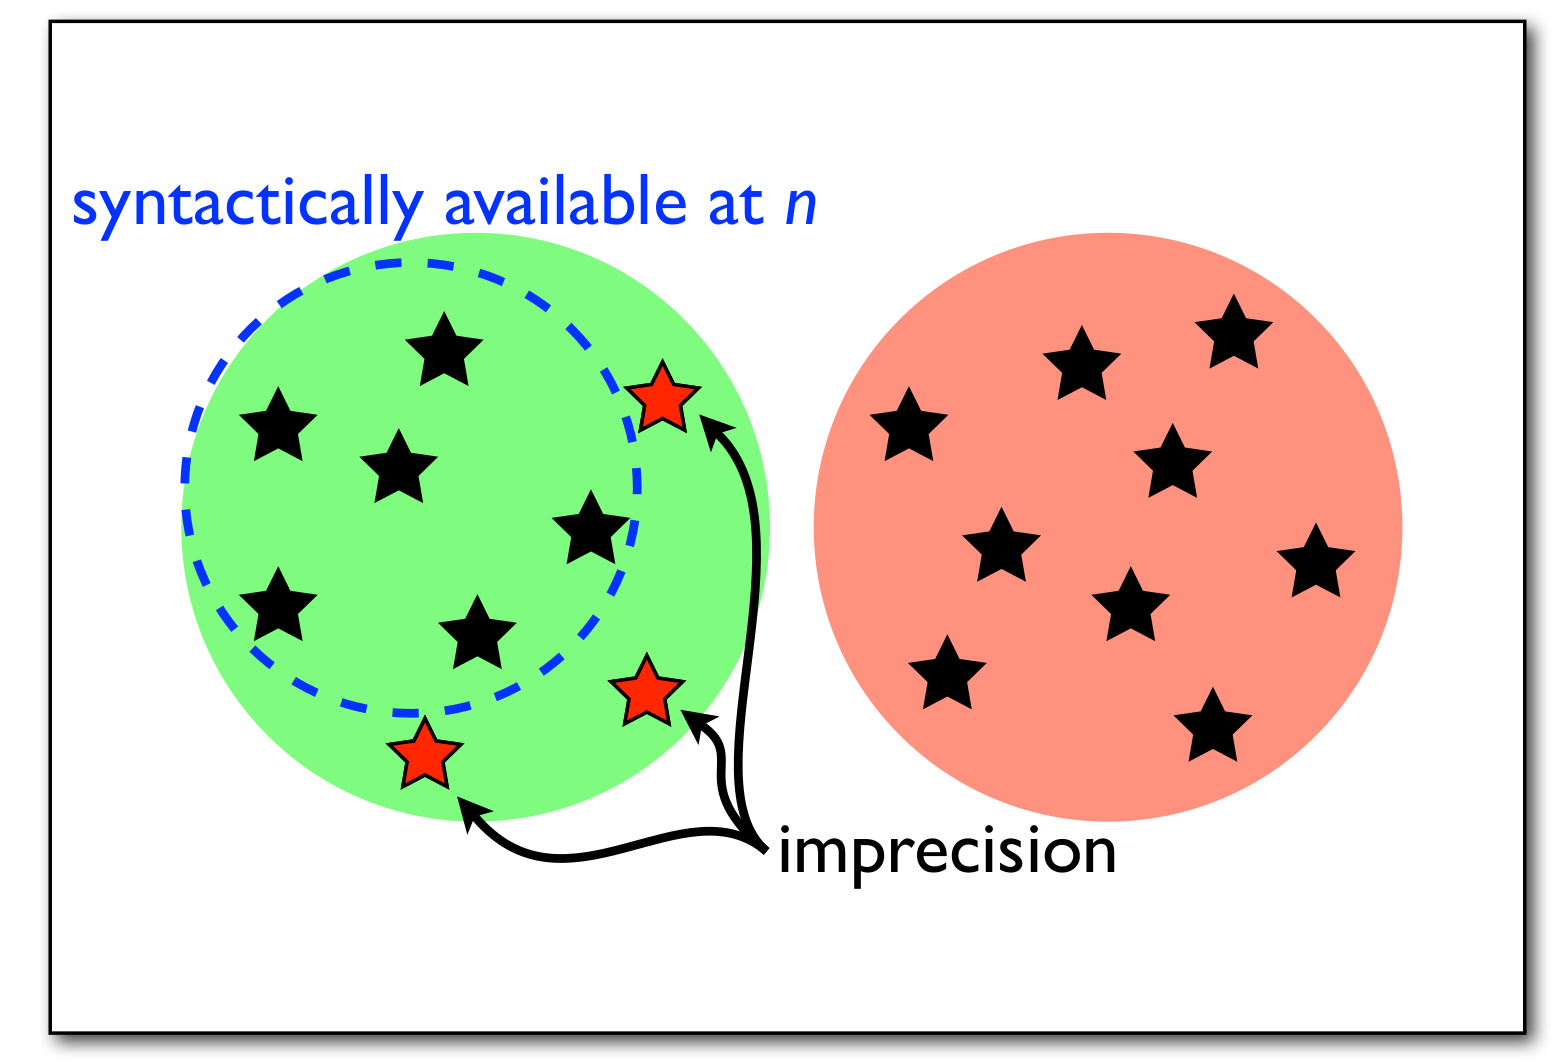
\includegraphics[width=\linewidth]{p6.png}
	\caption{Semantic vs. syntactic}\label{fig:p6}
	\endminipage
\end{figure}


\subsection{Summary}


\begin{center}
	\begin{tabular}{|c|c|}
		\hline Direction                         & Forward                                           \\
		\hline Domain                            & Sets of expressions                                    \\
		\hline Meet operator                     & \( \cap \)                                          \\
		\hline Top(T)                            & Universal Set                                             \\
		\hline Bottom                            & $\phi$                                     \\
		\hline Boundary condition                & $\mathrm{OUT[ENTRY]} = \phi$                          \\
		\hline Initialization for internal nodes & $\mathrm{OUT[B]} = T$                             \\
		\hline Finited escending chain?          & \checkmark                                          \\
		\hline Transfer function                 & $f_b(x) = \mathrm{Gen}_b \cup (x - \mathrm{Kill}_b)$ \\
		\hline Monotone\&Distributive?           & \checkmark                                          \\
		\hline $\mathrm{Kill}_b$ & all E such that block b defines a variable in E \\
    \hline $\mathrm{Gen}_b$ & all E such that block b evaluates E and doesn’t later kill it \\
    \hline
	\end{tabular}
\end{center}